\chapter{Einleitung}
\label{chap:einleitung}
In einer Welt, die sich mit rasanter Geschwindigkeit digitalisiert, suchen die Menschen stets nach Wegen, um die Komplexität des modernen Lebens zu bewältigen. Diese Digitalisierung hat eine stetig wachsende Sehnsucht nach der Vorhersage zukünftiger Ereignisse hervorgebracht - sei es in der Wirtschaft, der Gesundheitsbranche oder auch im Bereich des Dienstleistungssektors wie dem Hotelgewerbe. Es ist ein Streben nach Präzision, ein Bestreben, aus Daten und Mustern eine Art Kristallkugel zu formen, um die Zukunft vorhersagen zu können.
\newline
\newline
Albert Einstein hat es sehr treffend formuliert: 
\begin{zitat}
    If you want to know the future, look at the past. \cite{AE_zitat}
\end{zitat}
Dieser Gedanke illustriert die gängige Annahme, dass die Vergangenheit Hinweise auf die Zukunft liefern kann. Es ist interessant anzumerken, dass dieses Zitat auch als Titel eines Buches von Einstein dient, welches seine philosophischen Ansichten zur Zeit, Raum und Vorhersage behandelt.
\newline
\newline
Doch was passiert, wenn diese Vergangenheitsdaten nicht verfügbar sind oder nicht genutzt werden können? In Branchen wie der Hotelindustrie, die oft noch auf traditionelle, statische Preisstrategien zurückgreifen, stellt sich die Frage, wie eine effektive Vorhersage ohne spezifische historische Daten möglich ist. 
\newline
\newline
Es wird immer deutlicher, dass ein dynamischerer Ansatz im Hotelwesen erforderlich ist, um die Umsatzoptimierung durch Revenue Management zu steigern. Dies erfordert die Anpassung von Preismodellen an sich ändernde Nachfrage und andere Einflussfaktoren. Eine mögliche Lösung liegt in der Verlagerung der traditionellen Rolle des Revenue Managements auf Modelle, die auf breiteren Datenquellen und fortgeschrittenen Methoden des maschinellen Lernens basieren.
\newline 
\newline
Die Suche nach einem solchen Modell, das ohne die spezifischen Vergangenheitsdaten eines bestimmten Hotels auskommt, bildet das Herzstück dieser Forschungsarbeit. Der Fokus liegt darauf, alternative Datenquellen zu erkunden und innovative Ansätze zu entwickeln, um Prognosen und Entscheidungsgrundlagen für das Revenue Management in der Hotellerie zu schaffen. Ziel ist es, dass diese nicht ausschließlich auf vergangenen Daten eines spezifischen Hotels basieren, sondern auf einer Vielzahl von allgemeinen, zugänglichen Informationen und fortschrittlichen Analysemethoden beruhen. Es geht darum, einen Weg zu finden, wie Hotels, selbst ohne ihre spezifischen vergangenen Daten, zukünftige Entscheidungen im Bereich des Revenue Managements treffen können, um ihre Leistung zu optimieren und ihre Wettbewerbsfähigkeit zu stärken.

\section{happyhotel}
\label{sec:happyhotel}
Die vorliegende Masterthesis fängt mit einem umfassenden Überblick über die Firma happyhotel an. In diesem ersten Kapitel wird eingehend auf die fundamentale Idee und das herausragende Produkt von happyhotel eingegangen, welches einen signifikanten Beitrag zur Weiterentwicklung der Hotelbranche leistet.
\newline
\newline
Im Anschluss wird der Fokus auf das gegenwärtige Vorgehen des Unternehmens, der Dynamischen Preisgenerierung, gelegt. Diese fortschrittliche Methode, die auf einer Künstlichen Intelligenz und umfassender Datenanalyse basiert, ermöglicht es happyhotel, in Echtzeit auf auf den momentanen Markt zu reagieren und optimale Preise für Hotels zu generieren.
\newline
\newline
Abschließend wird in diesem einführenden Kapitel die zugrunde liegende Problematik hervorgehoben, die den Ausgangspunkt dieser Arbeit bildet. Dabei wird der Fokus auf eine Herausforderung gerichtet, die mit der Dynamischen Preisgenerierung einhergeht. Diese Problematik dient als Basis für die nachfolgende Analyse und Forschung, die darauf abzielt, innovative Lösungsansätze und Optimierungen im Rahmen der Preisstrategie von happyhotel zu entwickeln.

\subsection{Das Unternehmen}
\label{subsec:Unternehmen}
Die Firma happyhotel wurde im Jahr 2019 von den drei Gründern Sebastian Kuhnhardt, Marius Müller und Rafael Weißmüller gegründet. Sie wollten wie der Name schon vermuten lässt Hotels glücklicher machen. Angefangen hat es mit der Erkenntnis von Sebastian,  dass sich viele Hoteliers nicht mit der Dynamischen Preisgestaltung beschäftigen. Meist vertrauen diese Hoteliers einfach auf ihr Bauchgefühl, welcher Preis zur momentanen Situation passen könnte oder passen ihre Preise gar nicht an. 
\newline
\newline
Somit stellten sie sich die Fragen: 
\begin{itemize}
    \item Wie können die Preise für die Übernachtung in einem Zimmer besser vorausgesagt werden?
    \item Wonach sollten sich die Preise richten und wie kann man sie bestimmen?
\end{itemize}

Eine Lösung musste her um mehr Dynamik in die Preisgestaltung zu bringen. Sie erschufen die Software happyhotel ein Revenue Management System. Mit happyhotel kann der Hotelier sein gesamtes Hotel analysieren und Ihm werden Preisvorschläge für seine Zimmerkategorien generiert um mehr Umsatz zu erzeugen.
\begin{figure}[h]
    \centering
    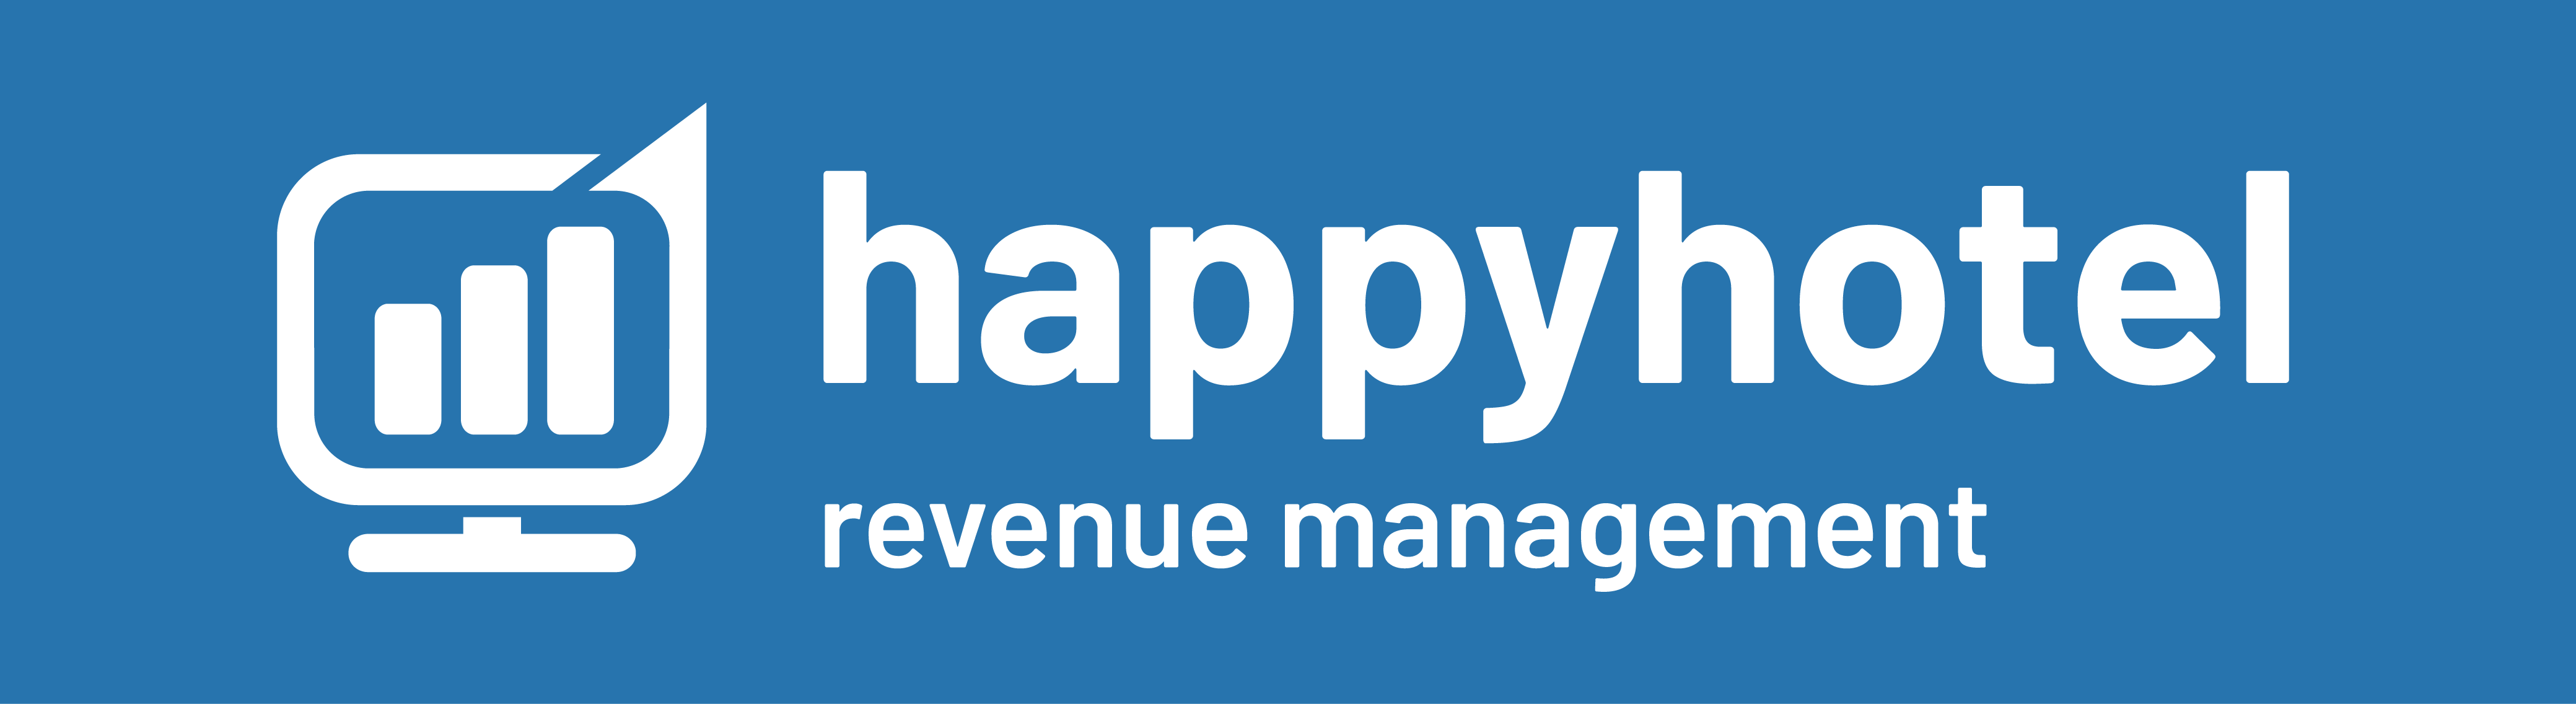
\includegraphics[width=0.5\textwidth, center]{happyhotel.png}
    \caption[happyhotel]{happyhotel}
    \label{img:happyhotel}
\end{figure}

\subsection{Dynamische Preisgenerierung}
\label{subsec:Preisgenerierung}
Wie im vorherigen Kapitel erwähnt, fokussiert sich happyhotel auf die dynamische Preisgenerierung. Um diese Preise zu generieren, braucht es vor allem zwei Sachen:
\begin{itemize}
    \item Die Daten des Hotels, wie zum Beispiel Buchungen
    \item Ein Vorgehen, um aus den gesammelten Daten Preise zu generieren
\end{itemize}

Die Daten bekommen sie aus den verschiedensten Quellen. Sogenannte Property Management Systeme kurz \emph{PMS}, sind Systeme, um ein Hotel zu verwalten. In diesen Property Management Systemen können Hotels zum Beispiel ihre Zimmer verwalten oder aber auch Buchungen anlegen und pflegen. Mit den Herstellern dieser Property Management Systeme arbeitet happyhotel zusammen, um an die Daten des Hotels zu gelangen. 
\newline
Wenn Daten vorhanden sind, braucht es ein Vorgehen, um aus den Daten einen Preis zu generieren. Dazu ist happyhotel auf die folgenden zwei Ideen gekommen:
\begin{itemize}
    \item Buchungskurvenmodell
    \item Kombination aus RevPAR und Buchungskurvenmodell
\end{itemize}

Das Buchungskurvenmodell war die erste Idee von happyhotel. Bei dem Buchungskurvenmodell wird die Vergangenheit angeschaut, um das zukünftige Buchungsverhalten vorherzusagen. Ziel dabei ist es, die Auslastung für einen Tag vorherzusagen, um anhand dessen einen akkuraten Preis zu bestimmen. 
\newline
\newline
Da sich bei dem Buchungskurvenmodell einige Schwächen aufgezeigt haben, wurde ein neues Modell erschaffen, um den Schwachstellen entgegen zu wirken. Es sollte nun der RevPAR-Wert vorhergesagt werden und mit dem Buchungskurvenmodell angepasst werden. RevPAR steht dabei für Revenue per Available Room. Auch bei diesem Modell wird sich die Buchungshistorie des Hotels angeschaut, um dann den zukünftigen Umsatz pro verfügbarem Zimmer vorherzusagen, und darauf basierend den endgültigen Preis zu ermitteln.
\subsection{Momentane Problematik}
\label{subsec:problematik}
Wie es Albert Einstein treffend formulierte: Soll die Zukunft vorhergesagt gesagt werden, so sollte sich die Vergangenheit angeschaut werden. Auf diesem Grundprinzip ist happyhotel auch vorgegangen, sie schauen sich bei beiden Ansätzen die Vergangenheit an, um dann Prognosen über die Zukunft zu generieren. 
\newline
\newline
Doch was passiert, wenn die Daten der Vergangenheit nicht vorhanden sind? Dies kann zum Beispiel passieren, wenn ein Hotel erst in der Zukunft öffnet und noch über keinerlei Daten verfügt. Auch dieses Hotel soll mit adäquaten Preisvorschlägen gefüttert werden.
Die soeben beschriebene Situation ist ein generelles Problem im Machine Learning Bereich. Es kommt nicht allzu selten vor, dass keine Vergangenheitsdaten aus den unterschiedlichsten Gründen vorliegen. Dieser Problematik soll in dieser Arbeit auf dem Grund gegangen werden. 
\newline
\newline
Ziel dieser Arbeit ist es,  ein Modell zu entwickeln, welches Preisempfehlungen für ein Hotel liefert, für das es bisher noch keine Vergangenheitsdaten gibt. Dieses Modell soll dann für folgende zwei Szenarien genutzt werden können:
\begin{itemize}
    \item Neue happyhotel Kunden ohne Daten
    \item Nachfrageeinschätzung für bestimmte Märkte
\end{itemize}
\section{Vorgehensweise}
\label{sec:Vorgehensweise}
Vor dem Eintauchen in die Lösung eines Problems ist es entscheidend, einen klaren Weg dorthin festzulegen. Antoine de Saint-Exupéry hat mit den Worten \emph{Ein Ziel ohne Plan ist nur ein Wunsch} treffend darauf hingewiesen, dass ein bloßes Ziel ohne einen durchdachten Plan lediglich eine vage Vorstellung bleibt. Das Verständnis und die Festlegung einer angemessenen Vorgehensweise sind daher der Schlüssel, um ein Problem effektiv anzugehen. Aufgrund dessen wird in dem folgenden Abschnitt dieser Arbeit auf die Vorgehensweise eingegangen. Zudem werden innerhalb dieser Sektion die Benchmark-Hotels ermittelt, an welchen getestet werden kann, ob die Vorgehensweise ein Erfolg war.  

\subsection{Vorgehen in der Datenwissenschaft}
\label{subsec:ds_vorgehen}
Ein Projekt, welches in der Datenwissenschaft (engl. Data Science) angesiedelt ist, beginnt in der Regel mit einem geschäftlichen Problem, so wie es auch in dieser Thesis der Fall ist. Sobald das Problem klar definiert ist, sollten ein oder mehrere Konzepte ausgearbeitet werden, wie das Problem gelöst werden kann. Diese Konzepte sollen als Leitfaden dienen, um das angestrebte Ziel zu erreichen. In der Regel ist es ratsam, mehr als ein Konzept auszuarbeiten, da so Ausweichmöglichkeiten festgelegt werden können, sollte ein Konzept nicht funktionieren. So werden auch in dieser Arbeit, in dem Kapitel \emph{\nameref{chap:konzepte}}, für das vorliegende Problem Konzepte ausgearbeitet und evaluiert. 
\newline
\newline
Mit der klaren Definition des Problems und der darauffolgenden Konzeption, kann der Datenwissenschaftler mit Hilfe des \emph{OSEMN}-Vorgangs die Problematik angehen \cite{Vorgehen_ds}. 
\newline
\newline
Der \emph{OSEMN}-Vorgang besteht aus den folgenden Elementen:

\begin{itemize}
    \item Obtian data (Erhalten von Daten)
    \item Scrub data (Daten reinigen)
    \item Explore data (Untersuchen von Daten)
    \item Model data (Modelldaten)
    \item Interpret results (Interpretieren von Ergebnissen)
\end{itemize}

\subsubsection{Obtian data}
Die wichtigste Ressource des 21. Jahrhundert besteht in den Daten, die zur Verfügung stehen. Dies erläuterte  Klaus Schwab, der Gründer des Weltwirtschaftsforums, mit seinen Worten: \emph{Die wertvollste Ressource des 21. Jahrhunderts sind nicht mehr Öl, sondern Daten}. Aufgrund dessen besteht der erste Schritt, nach der Evaluierung der Konzepte, in der Beschaffung der Daten. Es muss zunächst ein Überblick geschaffen werden. Zum Überblick gehören Informationen wie:

\begin{itemize}
    \item Welche Daten bereits vorhanden sind.
    \item Welche Daten eventuell noch intern neu erworben werden müssen.
    \item Welche Daten aus dem Internet gezogen werden können
\end{itemize}

Sobald die benötigten Daten vorliegen, kann mit dem nächsten Schritt fortgefahren werden.

\subsubsection{Scrub data}
Der nächste Schritt besteht darin, die Daten zu bereinigen. Zum Bereinigen der Daten gehört der Vorgang, mit dem die Daten in ein standardisiertes Format gebracht werden. Dazu gehört der Umgang mit fehlenden Daten, sowie die Korrektur von Fehlern und das Entfernen von sogenannten \emph{outlier} \cite{Vorgehen_ds}. Outlier sind Daten, welche im Verhältnis zu der gesamten Datenmenge aus der Reihe tanzen. 

\subsubsection{Explore data}
Die Datenuntersuchung oder auch Datenanalyse dient dazu, um mit den Daten vertraut zu werden und ein besseres Verständnis für die Daten zu gewinnen. Dies ist ein sehr wichtiger Schritt bei einem \emph{Data Science} Projekt, da nur dann ein gutes Ergebnis erzielt werden kann, wenn die Daten, mit den gearbeitet werden kann, verstanden sind. Das Verständnis über die Daten trägt zudem auch maßgeblich dazu bei, den richtigen Ansatz für die Modellierung zu finden.

\subsubsection{Model}
Nach dem Erforschen der Daten, kann ein \emph{Machine Learning} Modell eingesetzt werden. Es existieren viele verschieden Modelle, die meist für einen  speziellen Fall implementiert worden sind. Die Auswahl des Modells hängt ganz davon ab, welche Art von Problem gelöst werden soll und welche Daten vorhanden sind, um dieses Problem zu lösen. 

\subsubsection{Interpret results}
Der letzte Schritt besteht darin, die gesammelten Ergebnisse zu interpretieren. Dazu gehört die Entscheidung, ob die erzielten Ergebnisse gut oder schlecht sind. Meistens werden zur Hilfe der Entscheidung, ob die Ergebnisse gut oder schlecht sind, Diagramme, Grafiken und Tabellen erstellt. Es soll hier zudem auch entschieden werden, ob die Ergebnisse verwendet angewendet oder noch weiter geforscht werden muss. So entsteht ein Kreislauf, der mit dem Erstellen weiterer Konzepte startet und schlussendlich mit dem Interpretieren neuer Ergebnisse endet.

\subsection{Benchmark Hotels}
\label{subsec:bench_hotels}
Noch vor der Konzeptionierung zur eigentlichen Lösung der Problematik, sollten schon vorhandene Hotels in unserer Datenbank als \emph{Benchmark-Hotels} ausgesucht werden. Die Idee dahinter ist es, Hotels auszusuchen, bei denen viele Daten vorhanden sind und so zu tun, als wären gar keine Daten von diesen Hotels vorhanden. Mithilfe dieser Hotels sollen dann die ausgearbeiteten Konzepte im Kapitel \emph{\nameref{chap:konzepte}} validiert werden. Ein Konzept wird dann als gut empfunden, wenn es in der Lage ist, gute Preisvorschläge für die Benchmark-Hotels zu erzeugen.
\newline
\newline
Da nicht jedes Hotel, welches in der Datenbank vorhanden ist, in Frage kommt, wurden einige Kriterien aufgestellt, die ein Hotel erfüllen muss, um als ein Benchmark-Hotel gelten zu können. Diese Kriterien sehen wie folgt aus:

\begin{itemize}
    \item Haben Daten von mehr als zwei Jahren
    \item Haben einen Benutzer mit der Role \emph{Revenue Manager}
    \item Haben oft Preise geändert
    \item Haben oft vorgeschlagene Preise von happyhotel nicht angenommen
\end{itemize}

Die Begründung, warum die letzten drei Kriterien hinzu kamen, liegt darin, dass diese Hotels mit den Preisvorschlägen von happyhotel nicht zufrieden sind und vermutlich auch nur manuell \emph{Revenue Managment} betreiben. Die Hoffnung besteht darin, dass das Konzept nicht nur für Hotels ohne Vergangenheitsdaten gute Preisvorschläge liefert, sondern dass das Konzept auch verwendet werden kann, als Alternative zu den vorhandenen zwei Modellen, für Hotels, die noch manuell Dynamische Preise gestalten.
\newline
\newline
Es wurde zur Analyse der Hotels eine \emph{json}-Datei erstellt. Diese \emph{json}-Datei besteht aus einer Liste von einzelnen Objekten. Jedes Objekt innerhalb der Liste repräsentiert ein Hotel in der Datenbank. Ein Beispiel für diese \emph{json}-Datei könnte wie folgt aussehen:

\begin{lstlisting}[style=json, caption=Beispielhafte json-Datei,
    label=lst:json_file]
   [
    {
        company_id: "11111111111111",
        not_accepted_recs: 10,
        price_change_average: 5
    }
   ]
\end{lstlisting}

Das Feld \emph{not\_accepted\_recs} beschreibt dabei, wie viele Preisvorschläge das Hotel nicht angenommen hat, beziehungsweise ignoriert oder abgelehnt hat, und das Feld \emph{price\_change\_average} ist die durchschnittliche Preisänderung pro Tag. Anhand von diesen Informationen konnten zwei Hotels als Benchmark-Hotels ausgesucht werden.